% This is samplepaper.tex, a sample chapter demonstrating the
% LLNCS macro package for Springer Computer Science proceedings;
% Version 2.21 of 2022/01/12
%
\documentclass[runningheads]{llncs}
%
\usepackage[T1]{fontenc}
% T1 fonts will be used to generate the final print and online PDFs,
% so please use T1 fonts in your manuscript whenever possible.
% Other font encondings may result in incorrect characters.
%
\usepackage{graphicx}
% Used for displaying a sample figure. If possible, figure files should
% be included in EPS format.
%
% If you use the hyperref package, please uncomment the following two lines
% to display URLs in blue roman font according to Springer's eBook style:
\usepackage[utf8]{inputenc} % allow utf-8 input
\usepackage[T1]{fontenc}    % use 8-bit T1 fonts
\usepackage{hyperref}       % hyperlinks
\usepackage{url}            % simple URL typesetting
\usepackage{booktabs}       % professional-quality tables
\usepackage{amsfonts}       % blackboard math symbols
\usepackage{nicefrac}       % compact symbols for 1/2, etc.
\usepackage{microtype}      % microtypography
\usepackage{xcolor}         % colors
\usepackage{amsmath}        % AMS mathematical facilities
\usepackage{soul}           % Hyphenation for letterspacing, underlining, and more
\usepackage{natbib}         % Flexible bibliography support
\usepackage{graphicx}       % Enhanced support for graphics
\usepackage{amssymb}        % AMS symbol fonts m
\usepackage{algorithm}      % algorithms in pseudo-code
\usepackage{algpseudocode}  % algorithms in pseudo-code
\usepackage{color}          % Colour control
\usepackage{listings}       % Typeset source code listings
% \usepackage{emoji}          % Emoji support
\usepackage{fontawesome5}   % Font containing web-related icons
\usepackage{array}          % Extending the array and tabular environments
\usepackage{tikz}           % Create PostScript and PDF graphics
\usepackage{realboxes}      % \Colorbox can wrap verbatim, so \lstinline takes a background
\usepackage[official]{eurosym} % official style euro symbol 

\definecolor{ftgyellow}{HTML}{FFCD69} 
% --- palette (light, print-friendly) ---
\definecolor{ttlDirective}{HTML}{0033B3} % @prefix, a, true/false
\definecolor{ttlPredicate}{HTML}{871094} % CURIE predicates (hb:, dcterms:)
\definecolor{ttlIRI}{HTML}{0E7C66}       % <...> IRIs
\definecolor{ttlString}{HTML}{A31515}    % "literals"
\definecolor{ttlComment}{HTML}{6E6E6E}   % # annotations
\definecolor{ftgdarkblue}{HTML}{004C99}
\definecolor{ftglightblue}{HTML}{D4E1F5}
\definecolor{ftglightgreen}{HTML}{E3E7E2}
\definecolor{ftgdarkgreen}{HTML}{6D9656}
\definecolor{ftgyellow}{HTML}{FFCD69} 

\lstdefinelanguage{turtle}{
  sensitive=true,
  alsoletter={@:-},                       % so @prefix and hb:contextLink are single tokens
  morekeywords={a,@prefix,@base,true,false},
  morekeywords=[2]{hb:contextLink,hb:matchedActivity,hb:estimatedDurationMinutes,
                   hb:isConcurrent,hb:isDividable,dcterms:title,dcterms:description},
  morecomment=[l]{\#},
  morestring=[b]",
  moredelim=[s][\color{ttlIRI}]{<}{>},    % colours IRIs; also stops '#' inside them starting a comment
}
\lstset{
  language=turtle,
  backgroundcolor=\color{gray!20},
  % basicstyle=\fontfamily{pcr}\fontsize{7}{8}\selectfont, % Courier; 1st num=size, 2nd=line spacing
  basicstyle=\ttfamily\small,
  backgroundcolor=\color{gray!20},
  keywordstyle=\color{ttlDirective}\bfseries,
  keywordstyle=[2]\color{ttlPredicate},
  stringstyle=\color{ttlString},
  commentstyle=\color{ttlComment}\itshape,
  numbers=none,
  showspaces=false,
  showstringspaces=false,
  showtabs=false,
  frame=single,
  escapeinside={(*}{*)},
  rulecolor=\color{black},
  rulesepcolor=\color{gray},
  tabsize=2,
  captionpos=b,
  breaklines=true,
  breakatwhitespace=false,
  columns=fullflexible,
  % postbreak={},
  % breakindent=0pt,
}

\setlength{\fboxsep}{1.5pt} % tight padding for inline code chips
\renewcommand\UrlFont{\color{blue}\rmfamily}
% process model blue port
\newcommand{\dtriblue}{%
  \tikz[baseline=-0.5ex]{%
    \filldraw[draw=ftgdarkblue, fill=ftglightblue, line join=miter, line width=0.4pt]
      (-0.5em,0.3em) -- (0.5em,0.3em) -- (0,-0.3em) -- cycle;%
  }%
}
% process model green port
\newcommand{\dtrigreen}{%
  \tikz[baseline=-0.5ex]{%
    \filldraw[draw=ftgdarkgreen, fill=ftglightgreen, line join=miter, line width=0.4pt]
      (-0.5em,0.3em) -- (0.5em,0.3em) -- (0,-0.3em) -- cycle;%
  }%
}
% process model activity: rounded box, white fill, black outline
\newcommand{\rbox}{%
  \tikz[baseline=-0.5ex]{%
    \filldraw[draw=black, fill=white, line width=0.4pt, rounded corners=0.12em]
      (-0.45em,-0.33em) rectangle (0.45em,0.33em);%
  }%
}

% process model automated activity: rounded box, yellow fill, black outline
\newcommand{\rboxyellow}{%
  \tikz[baseline=-0.5ex]{%
    \filldraw[draw=black, fill=ftgyellow, line width=0.4pt, rounded corners=0.12em]
      (-0.45em,-0.33em) rectangle (0.45em,0.33em);%
  }%
}

% process model artifact: cut-corner (note) box, light green fill, dark green outline
\newcommand{\ccbox}{%
  \tikz[baseline=-0.5ex]{%
    \filldraw[draw=ftgdarkgreen, fill=ftglightgreen, line width=0.4pt]
      (-0.5em,-0.33em) rectangle (0.5em,0.33em);%
  }%
}

% process model split / join bar: solid dark-blue horizontal bar
\newcommand{\sjbar}{%
  \tikz[baseline=-0.6ex]{%
    \fill[ftgdarkblue] (-0.75em,-0.18em) rectangle (0.75em,0.18em);%
  }%
}
% \urlstyle{rm}
\allowdisplaybreaks % let long aligned equation blocks break across a page
\begin{document}
%
\title{CalendarBench: Benchmark Framework for Personal Scheduling in the Wild}
%
% \titlerunning{CalendarBench}
% If the paper title is too long for the running head, you can set
% an abbreviated paper title here
%
\author{Maani Beigy \inst{1,2}\orcidID{0000-0003-2963-3533} \and
Roy van den Munckhof\inst{1} \and \\
Laura Genga \inst{1,2}\orcidID{0000-0001-8746-8826}
\and \\
Pieter Van Gorp \inst{1,2}\orcidID{0000-0001-5197-3986}
}
%
\authorrunning{M. Beigy et al.}
% First names are abbreviated in the running head.
% If there are more than two authors, 'et al.' is used.
%
\institute{Eindhoven University of Technology, Eindhoven, the Netherlands \and
Eindhoven Artificial Intelligence Systems Institute, Eindhoven, the Netherlands
\email{
\{m.b.beigy,l.genga,p.m.e.v.gorp\}@tue.nl, \\
\{r.m.a.v.d.munckhof\}@student.tue.nl}
}
%
\maketitle              % typeset the header of the contribution
%
\begin{abstract}
Effective planning and managing personal time are associated with higher productivity and greater well-being. Improvements in health, happiness, and personal development depend on whether people allocate time to beneficial activities, which often requires adopting new routines that challenge existing habits. Planning when to perform each new activity and assessing its cognitive and physical demand is itself a burden. This challenge has motivated an increasing number of tools and techniques that automate personal scheduling, from constraint solvers to planners and intelligent personal assistants. However, no benchmark framework exists for personal scheduling in this knowledge-intensive setting, which is crucial to test and compare such personal scheduling methods on common ground before conducting studies on human participants. We address this gap with \textsc{CalendarBench}, a configurable benchmark framework that provides a knowledge-grounded persona-based simulation of a user's calendar and context trace. We use large language model (LLM) capabilities and graph retrieval augmented generation (GraphRAG) to enable dynamically generating recommended activities and evaluating any scheduled plan with a multi-objective human-centric metric. A scheduler of interest can be compared with state-of-the-art (SOTA) techniques using built-in configurable comparisons. We demonstrate such capabilities with an example benchmark experiment and testing with five SOTA models.

\keywords{Personal scheduling \and Benchmarking \and Knowledge graphs \and LLM \and RAG \and Human-centric optimization \and Behavior change}
\end{abstract}
%
%
%
\section{Introduction}
\label{section:introduction}

\begin{figure}[h]
    \centering
    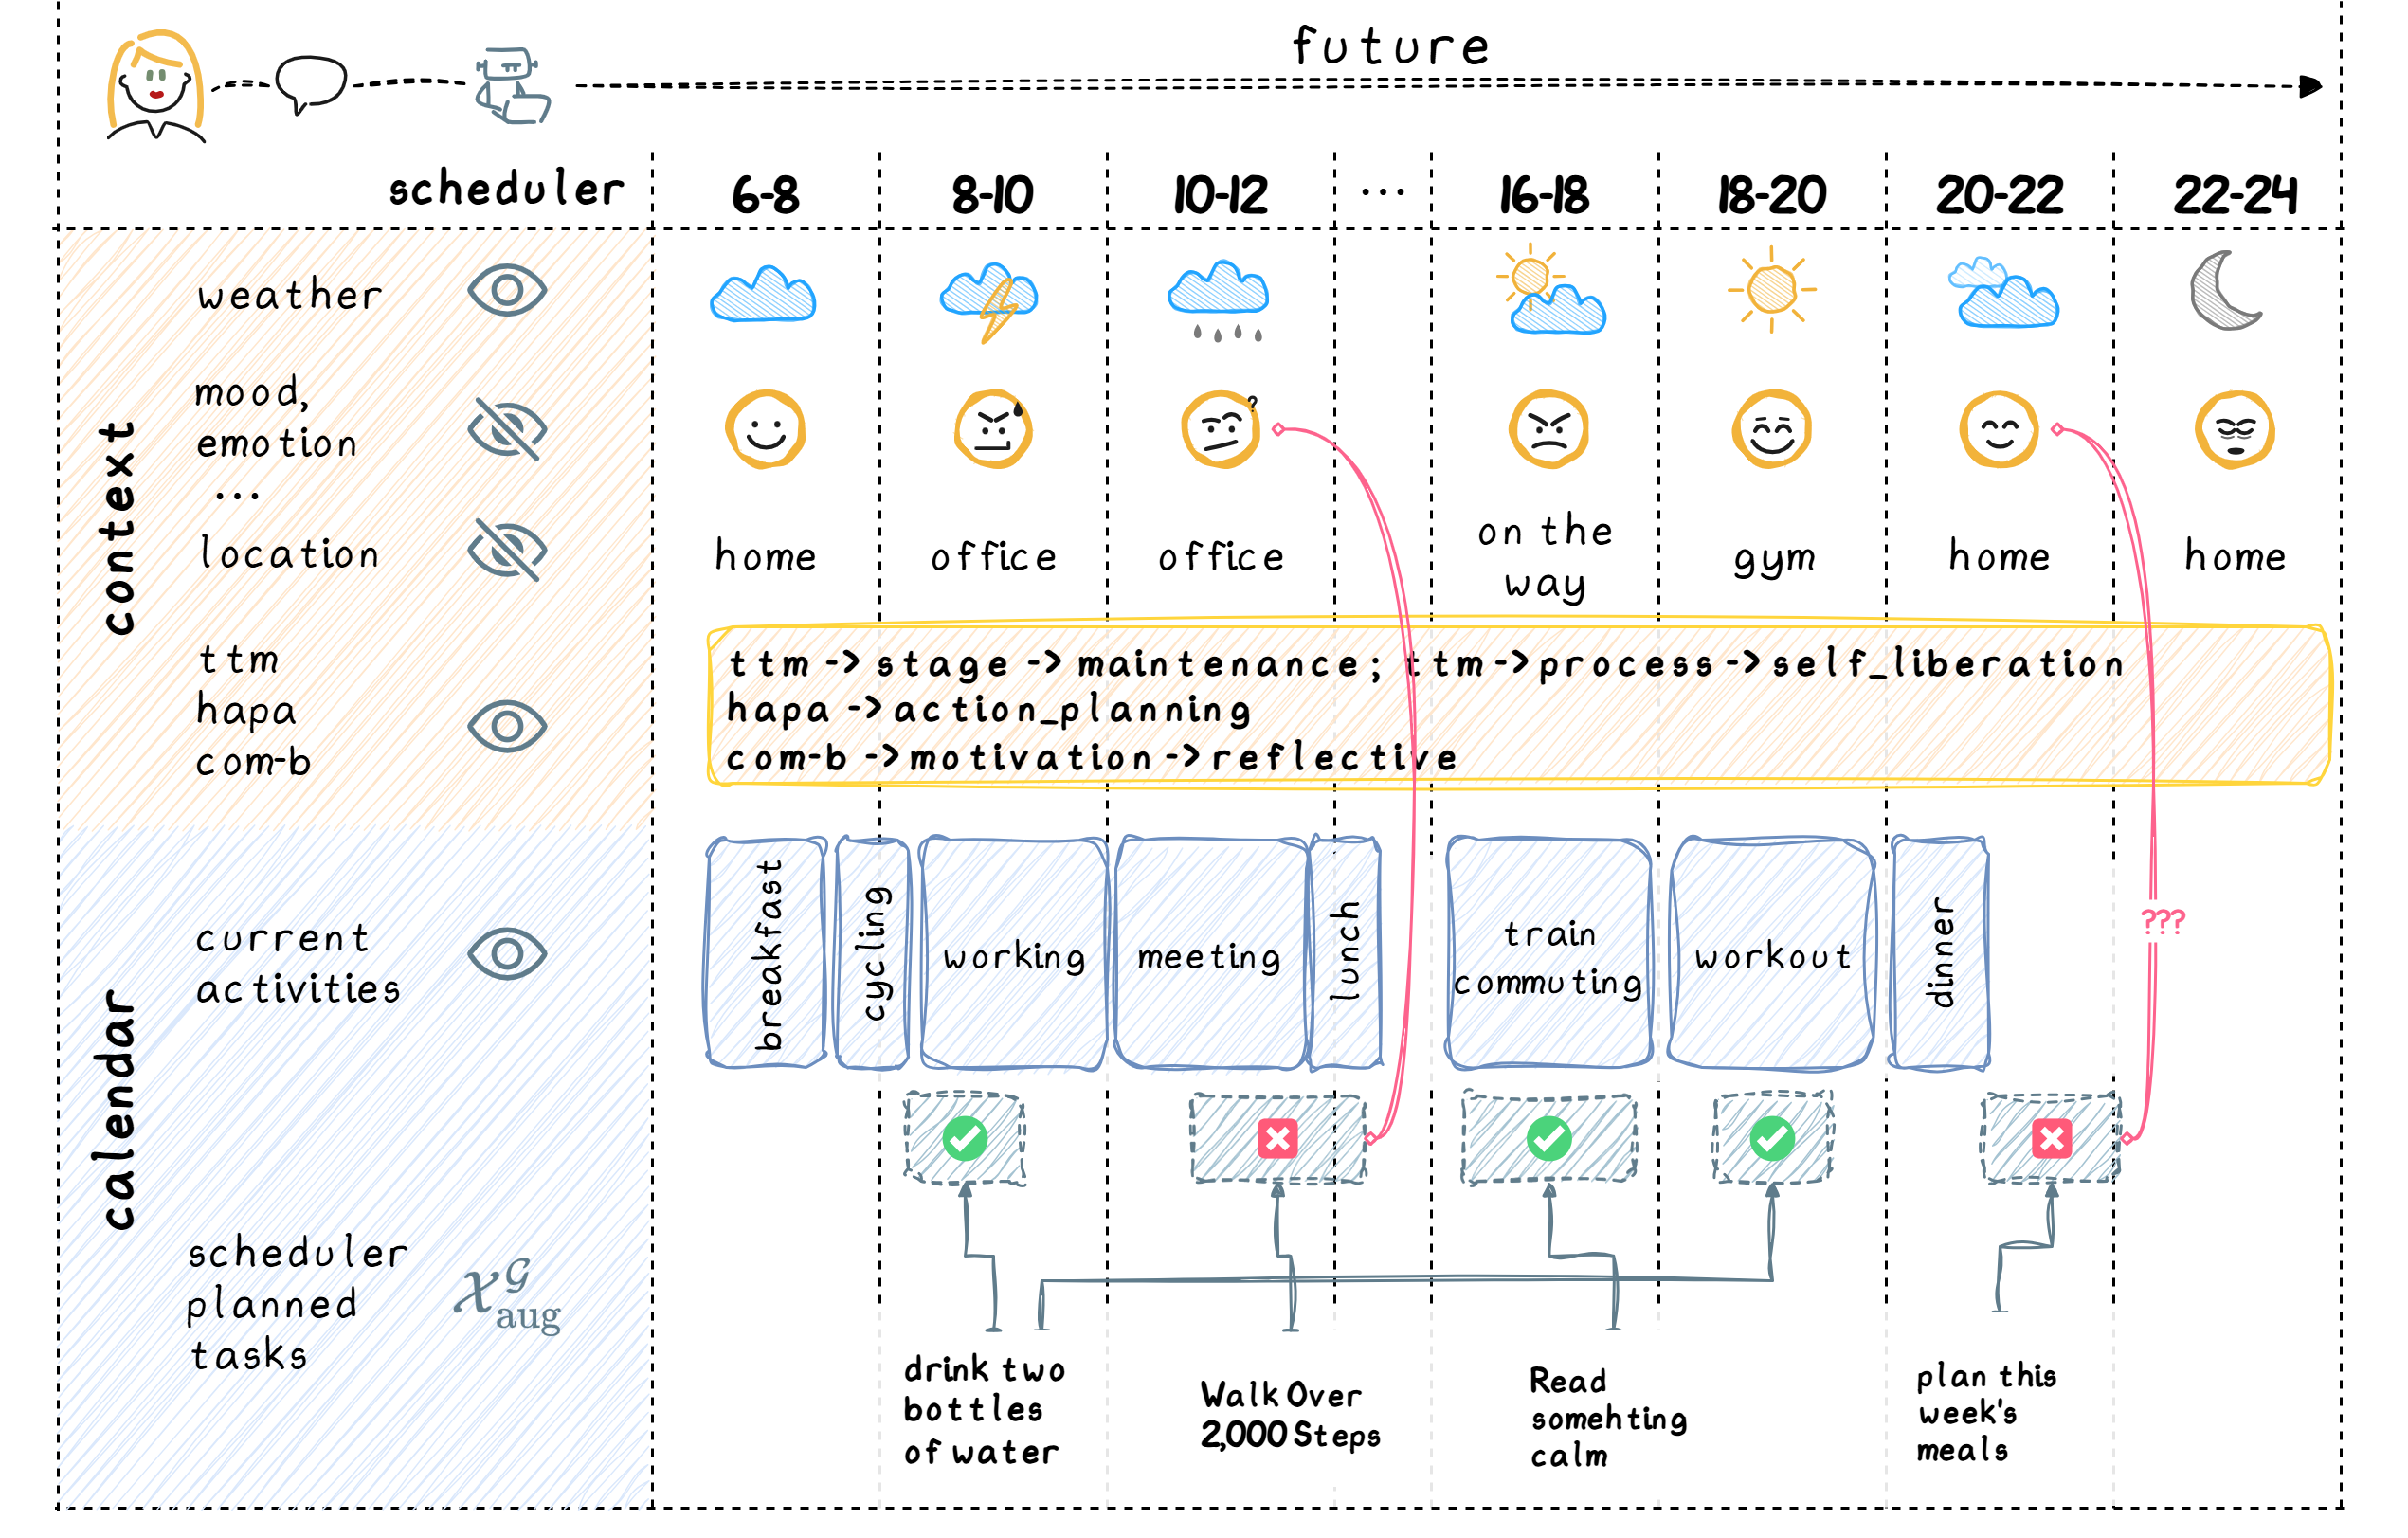
\includegraphics[width=\textwidth]{problem-large.png}
    \caption{
        Overview of personal scheduling problem. Given the calendar and context traces over a finite horizon, a scheduler augments the person's calendar ($\mathcal{X}^{\mathcal{G}}_{\mathrm{aug}}$) by placing given tasks (the dashed boxes) around existing activities. Experiment configurations determine if the scheduler observes some context (\faEye[regular]{:} weather, behavior-change states) while the rest are hidden (\faEyeSlash[regular]{:} location, mood).
    }
    \label{fig:problem-overview-large}
\end{figure}


There is growing societal and scientific interest in how people manage their time, since research shows that effective time management improves well-being and performance while reducing psychological distress \citep{does_time_management}. However, planning personal time is itself a decision-making burden \citep{kool_decision_2010}. Assessing the cognitive and physical demands of each activity and deciding when to perform it requires effort and thought from the same person who hopes to benefit from the plan. This burden is heaviest when someone wants to adopt activities and routines beyond the \textit{status quo} of daily life, either for productivity or for a healthier lifestyle \citep{wood_habits_2022}. 

\textit{Personal scheduling} methods address the problem of deciding when a person should perform a set of given tasks within the dynamic setting of daily life. It is a central feature of human-centric information systems such as mobile health applications, lifestyle and productivity tools, and intelligent personal assistants \citep{Li2024PersonalSecurity}. The problem differs from classical scheduling, such as job-shop and machine scheduling. In personal scheduling, the user is the sole resource and the objective combines temporal feasibility, satisfaction of preferences, cognitive and physical burden of tasks, and the evolving context and desires of the user (Figure~\ref{fig:problem-overview-large}). These human-centric factors, together with the uncertainties of real life, make personal scheduling notoriously difficult \citep{cpsat,Berry2011PTIME:Calendaring}. Interest in the problem has recently been revived, as advances in large language models (LLM) bring new methods to personal scheduling, including constraint solvers embedded in calendaring tools \citep{hao2025llmssolve}, LLM-based planners \citep{xie_travelplanner_2024,zheng_natural_2024,valmeekam_planbench_2023}, and coaching assistants \citep{james_toward_2025,shin_planfitting_2025,jorke_gptcoach_2025}.

The systems above, from digital calendars to intelligent assistants, are evaluated on ad-hoc tasks, fixed datasets, or subjectively, which makes it hard to measure progress or compare techniques. This mirrors the challenges seen in other HCI and AI domains before the introduction of benchmark suites, which historically catalyzed rapid advances by providing common tasks, standardized metrics, and evaluation settings  \citep{rein_gpqa_2024, hendrycks_mmlu_2021}, which have enabled reproducible, repeatable, and replicable evaluations \citep{ftgpm}. To the best of our knowledge, such a benchmark does not exist for personal scheduling, and we argue that a benchmarking framework is needed to support advancements in personal scheduling, providing a rigorous basis for measuring performance, comparing different approaches under controlled conditions. This is an essential step before conducting usability studies and clinical trials, as the scientific community prefers to evaluate interventions \textit{in silico} before trials on human participants \citep{user_simulation}.

We address this gap with \textsc{CalendarBench}, a configurable, knowledge-grounded benchmark framework and simulator that allows the researchers to design controlled experiments to test different scheduling methods and evaluate each with a multi-objective human-centric metric. In the rest of this manuscript we:  review related works (Section \ref{section:related_works});  present the benchmark framework (Section \ref{sec:method}); evaluate the  framework capabilities with an example benchmark experiment and test it with five SOTA models (Section \ref{sec:evaluation}) as proof-of-concept; and provide conclusions and possible future research directions (Section \ref{sec:conclusion}).  


\section{Related works}
\label{section:related_works}

Early calendaring assistants treated scheduling as a constraint problem on
candidate time slots, considering user preferences. PTIME models scheduling as a disjunctive temporal problem with preferences (DTPP), maps its temporal constraints into preference criteria as a multi-criteria DTPP, and solves that with a branch-and-bound search inside the multi-criteria search algorithm \citep{Berry2011PTIME:Calendaring}. It learns the user's preference weights from a short setup step and keeps updating them online with SVM learning. CMRadar is one of the first end-to-end calendar management
systems that parses scheduling emails into a normalized template format,
enables negotiations with other users, and employs the Ozone scheduler for core optimization \citep{Modi2005CMRadar:Management}. Both of these approaches are based on temporal constraint networks, where consistency can be decided in polynomial time when each pair of time points carries a single interval, but it soon becomes NP-hard once the constraints carry several intervals \citep{Dechter1991}. A recent study in the line of constraint programming, TaskFlow Optimizer \citep{cpsat}, models personal scheduling as a constraint optimization problem and solves it with the CP-SAT solver from Google OR-Tools. It provides a library of customizable soft-constraint templates, such as working hours, energy profiles, task grouping, and breaks, combined in a single weighted objective.

% Together, these systems established calendaring as a preference-aware constraint problem and showed how to model and solve it in practice. Since their objective is mainly preference satisfaction for a fixed set of requested meetings, these works do not account for the user's evolving context and requirements, the non-stationary temporal patterns in everyday life, or the aspects of calendaring beyond preference, such as how fully a schedule covers the recommended tasks a person wants to adopt, how evenly the burden of those tasks is distributed across the calendar, and how well each task fits user's context. They also treat the user as stationary and treat user preferences statically \citep{cpsat}.
% , and even PTIME, whose preference weights are refined online, fits a stationary preference model rather than tracking behavior and context that drift over time.
% We build on constraint-based formulation of these studies and extend the objective to the uncovered dimensions, while modeling preferences and routines as non-stationary across the scheduling horizon.

% A more recent neuro-symbolic line of
Recently, researchers have integrated a learning component with an exact solver, such as mixed-integer linear programming (MILP) for travel itineraries in TTG \citep{ju2024ttg} and SMT solvers for natural-language (NL) planning queries \citep{maas_generating_2026,hao2025llmssolve}. In addition, interactive designs have been introduced which keep the user in the loop, allowing them to adjust and relax constraints step by step, so that the solver only handles a smaller subset  \citep{bilbily_space_2021}.
% These are solver-based planning methods, and approaches of this kind are among the methods we want to be able to evaluate.

Recent studies have explored the capabilities of LLMs in personal scheduling and have tested it through standardized and reproducible benchmarks. TravelPlanner defines multi-day itinerary planning as a sandboxed problem with a set of nearly four million records and 1{,}225 annotated query-plan pairs, and evaluates a plan by commonsense and hard-constraint pass rates \citep{xie_travelplanner_2024}. NaturalPlan covers trip planning, meeting planning, and calendar scheduling as NL tasks in a fixed set of 3{,}600 instances, gives the model the information it needs in advance from Google Flights, Maps, and Calendar, and grades each plan by exact match against a reference solution \citep{zheng_natural_2024}. PlanBench grades LLM plans in the classical Blocksworld and Logistics domains, using a domain-independent planner and validator that work from the planning domain definition language (PDDL) specification \citep{valmeekam_planbench_2023}. CalBench is a benchmark for multi-agent calendar scheduling, where several agents hold private calendars and coordinate to place a stream of shared meetings, and scores coordination quality, communication efficiency, fairness, and privacy leakage \citep{calbench}. 

% None of these establishes its tasks in a configurable domain ontology nor scores an evolving single-user calendar with a multi-objective human-centric metric.

% Instead, we evaluate scheduling as a sustained evolving problem, where new recommended activities should be added to the user's calendar repeatedly and dynamically over a horizon, rather than one-shot placement.

Digital health researchers have approached the personal scheduling problem through conversational coaching agents that ask the user about goals, free time, and obstacles, then return a structured activity plan. Examples include LLM-driven goal and plan generation \citep{james_toward_2025}, PlanFitting for personalized exercise planning \citep{shin_planfitting_2025}, and GPTCoach, which adds wearable data to motivational physical-activity plans \citep{jorke_gptcoach_2025}. These systems successfully move the burden of planning from the user to the agent, yet they are tested mainly on participants' subjective experience, in clinical or usability studies. 
% Such evaluations look at health outcomes or user experience and pay little attention to whether the generated plans are well-timed and temporally feasible in the user's daily routine.


% CalBench focuses on decentralized coordination and the trade off between coordination and privacy among different users, while we focus on the single-user setting, where one person's time is the only resource being scheduled, and the main problem is sceduling activities that person wants and fitting them into their evolving routine and context.

% Together, a versatile benchmark suite for personal scheduling is missing. Such a benchmark would need to (i) generate everyday calendar events and user's context in a configurable way, (ii) generate recommended tasks and plans at runtime, (iii) be able to test schedulers that add behaviors that go beyond the status quo, as in lifestyle and mHealth, while keeping the schedule temporally feasible, (iv) score any solver automatically, with no manual annotation or checks, and (v) go past zero- or few-shot calendaring toward sustained coaching.

To the best of our knowledge, no benchmark has been proposed to evaluate personal scheduling frameworks against standardized metrics and evaluation settings.
%captures the big picture for personal scheduling. 
% as we expect to (i) generate recommended or desired tasks at runtime; (ii) generate non-stationary traces of context and calendars in a configurable way, (iii) test schedulers that add behaviors beyond the status quo, as in lifestyle and mHealth, while keeping the calendar temporally feasible, (iv) score any method automatically on a multi-objective setting, with no manual annotations, and (v) go past one-shot calendaring and approach toward iterative longitudinal planning for learning methods such as reinforcement learning (RL). 
We address this gap with a configurable system that couples LLMs with Graph Retrieval-Augmented Generation (RAG) based on ontologies \citep{zhang_survey_2025} to enable a versatile environment.

% \begin{figure}[h]
%     \centering
%     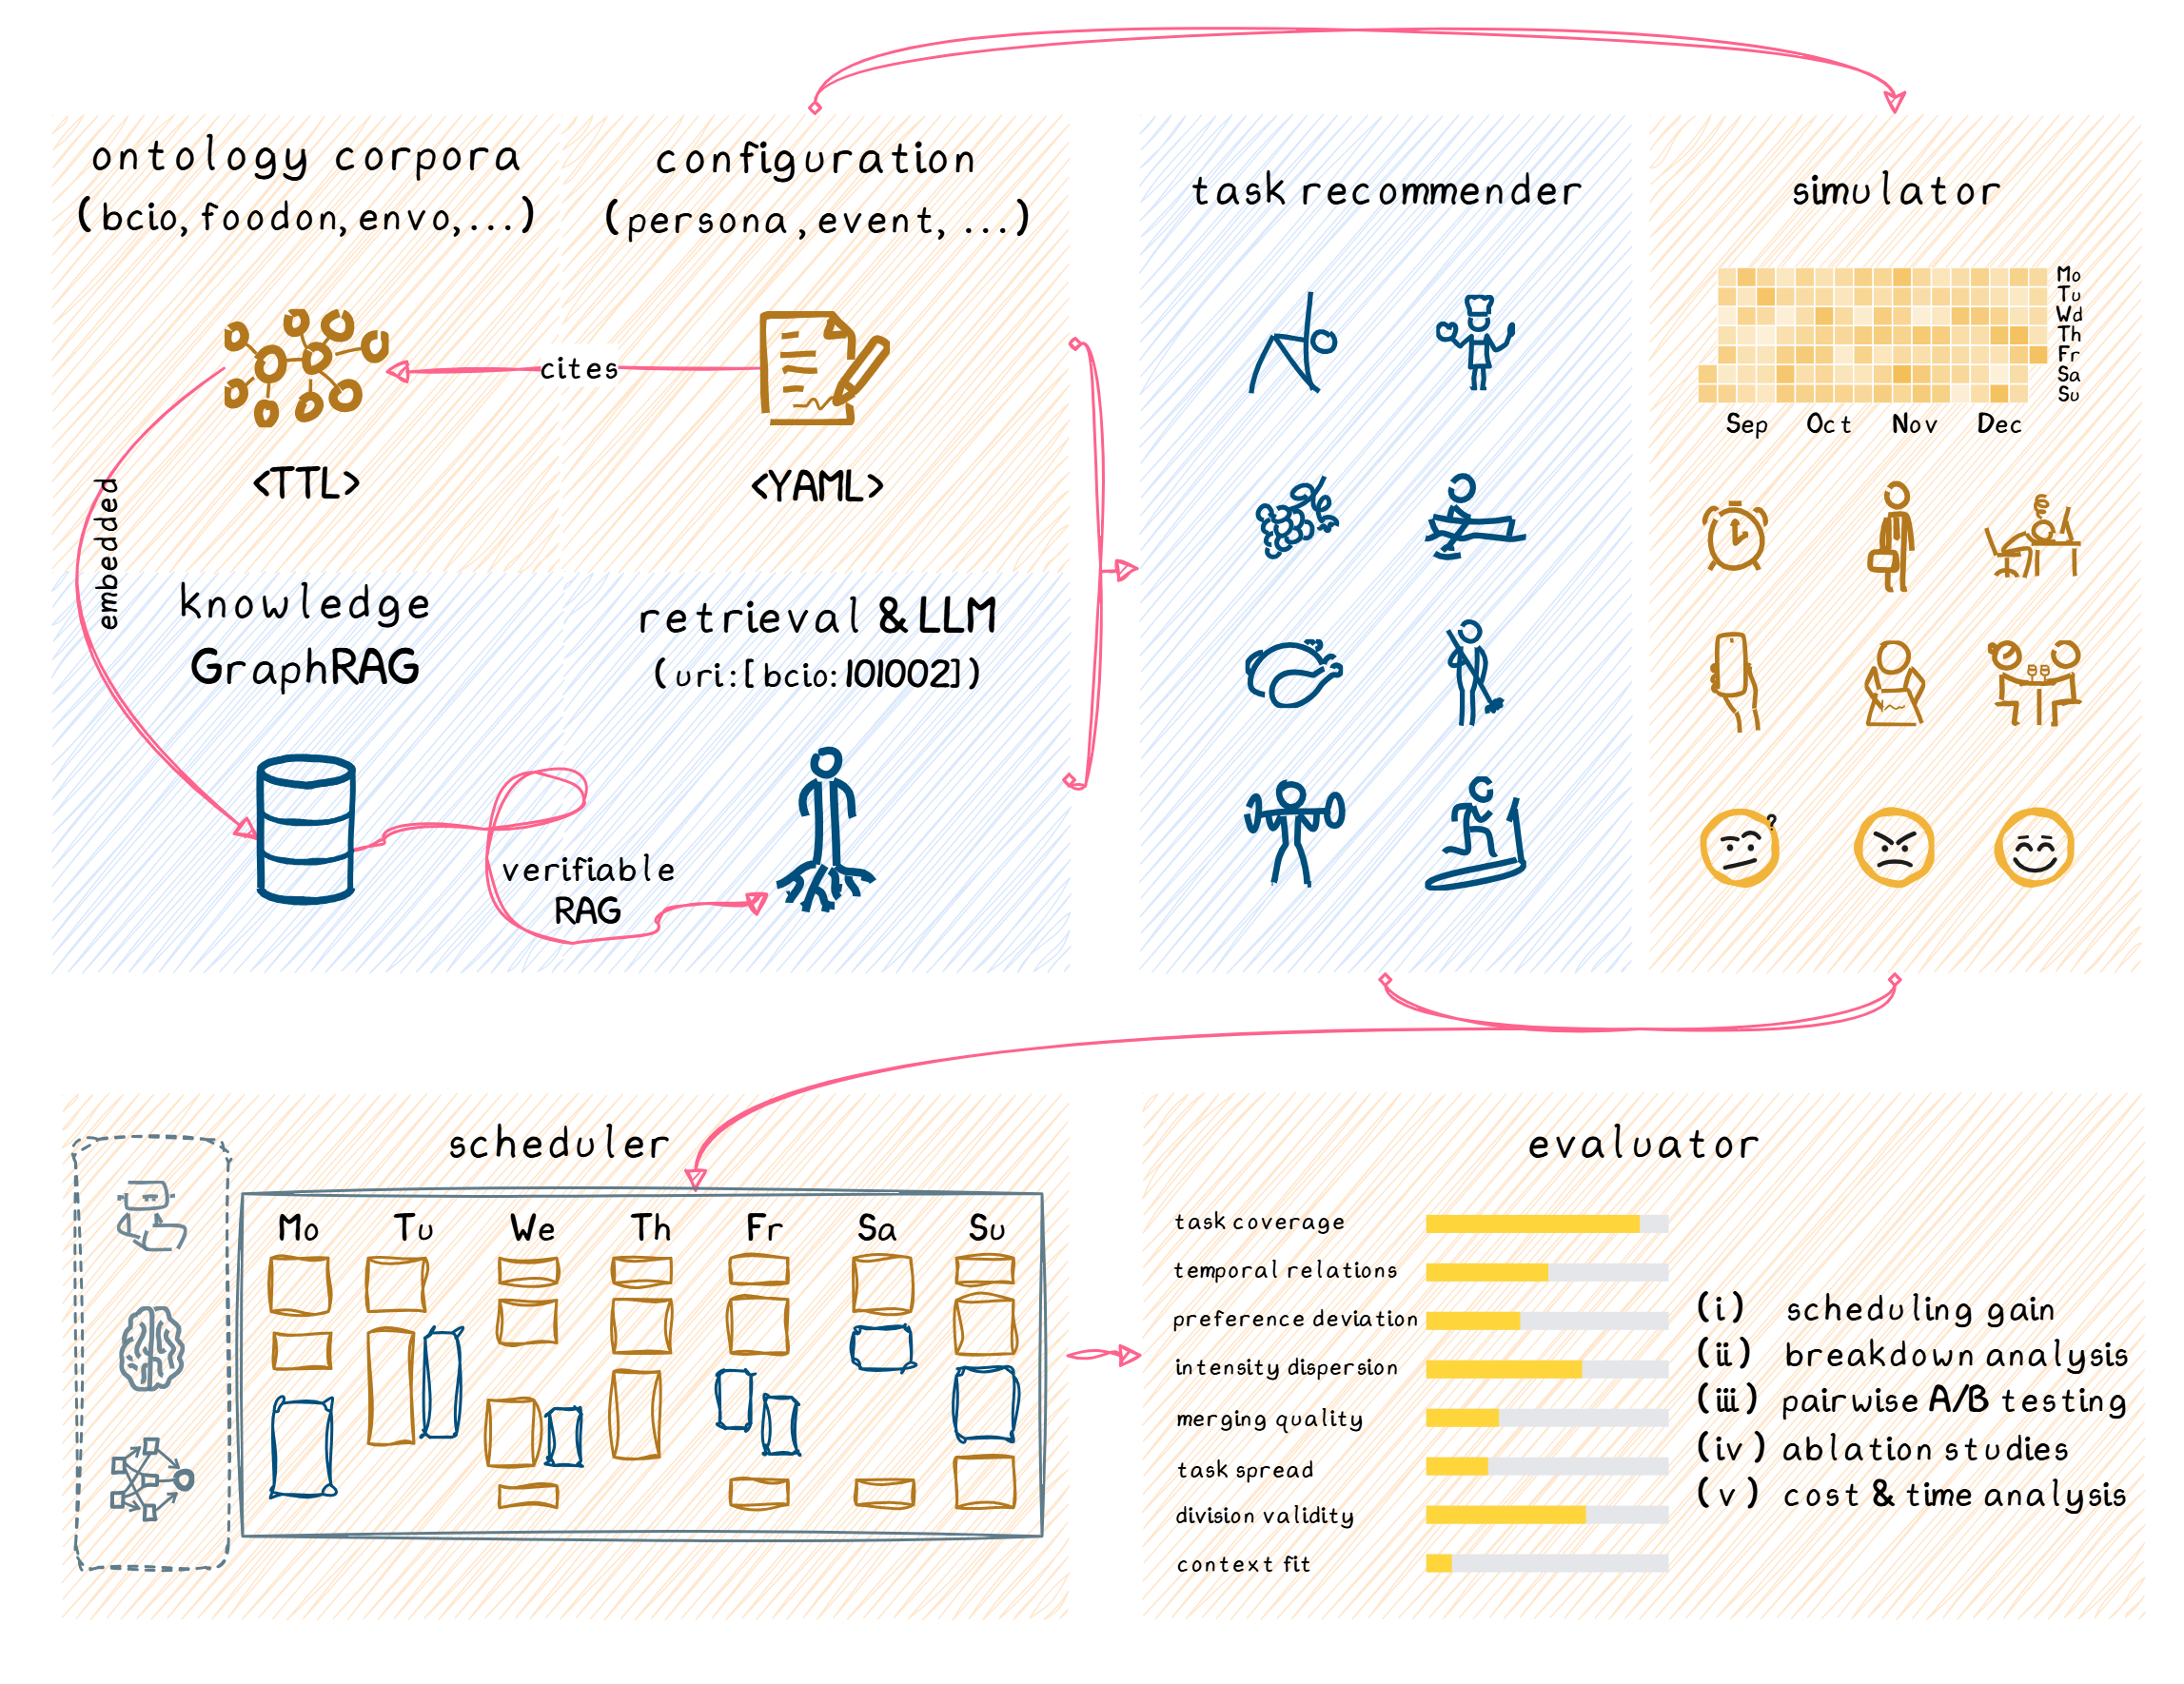
\includegraphics[width=\textwidth]{components.png}
%     \caption{
%          Graphical representation of the personal calendar scheduling benchmark. It consists of eight main components: ontology corpora and data, GraphRAG database, retrieval and LLMs, configurations, task recommender, simulator, scheduler solutions, and evaluator. These components are described in Section~\ref{sec:architecture}, with each playing are role in preparing knowledge-base, configuring simulation environment, defining scheduling problem, setting up solution methods, or reporting evaluation results.
%     }
%     \label{fig:components}
% \end{figure}
\section{Methods}
\label{sec:method}
We developed \textsc{CalendarBench} following the design science research methodology \citep{wieringa_design_2014}. First, we identified the problem and derived the requirements from the literature on personal scheduling (Section~\ref{section:related_works}). Table~\ref{tab:req} pairs each requirement with the design decision that satisfies it. The remainder of this section presents %the design of the artifact, 
a formalization of personal scheduling concepts (Section~\ref{sec:math}), followed by the workflow showcasing the working logic of the benchmark (Section~\ref{sec:architecture}). 

% The implementation is method-agnostic, so it admits schedulers such as LLM-based pipelines, reinforcement learning (RL) and  heuristics. A scheduler can read a calendar of already-planned events, a set of recommended tasks, and a partial observation of user contextual states, and returns an augmented calendar in which each task is placed in a free slot or merged into a compatible eventuality.

\subsection{Problem formulation}
\label{sec:math}

We formulate every calendar event, contextual state (e.g. mood, location, stress, energy), and recommended task (i.e. to-do), uniformly as an \emph{eventuality} \citep{GALTON200525}, which is a labeled interval $e=(\eta,\tau_s,\tau_e)$ with label $\eta$ from a vocabulary $\mathcal{V}$ and its times $\tau_s\le\tau_e$ within a timescale $T_{\mathcal{G}}$ of granularity $\mathcal{G}$, such as $\texttt{hour}$, $\texttt{day}$, or $\texttt{week}$, with horizon length $|T_{\mathcal{G}}|$. A coarser scale groups finer epochs, as with the day scale $T_{\mathcal{D}}\preceq T_{\mathcal{G}}$, when each day-epoch is a union of the finer $\mathcal{G}$-epochs within it \citep{Bettini2009}. We denote the interval of $e$ by $I(e)=[\tau_s,\tau_e)$, and the gap between two eventualities by $\rho(e,e')=\max\{0,\,\tau_s'-\tau_e,\,\tau_s-\tau_e'\}$, being the idle time between $I(e)$ and $I(e')$, which is zero when they overlap. Let \emph{trace} be a time-ordered sequence of eventualities. We define \textit{calendar trace} $\mathcal{X}^{\mathcal{G}}$ as a trace consisting of eventualities from an activity ontology $\mathcal{O}^{x}$, and a \textit{context trace} $\mathcal{Z}^{\mathcal{G}}$ as a trace consisting of eventualities from a context ontology $\mathcal{O}^{z}$. 
% We used a total function for ontology lookup \citep{BaaderDLHandbook2007} with a configured
% default $d$, so $\bigl[\mathcal{O}(\eta,a)\bigr]_{d}=\mathcal{O}(\eta,a)$ when
% $\mathcal{O}(\eta,a)\ne\bot$ and $d$ otherwise.

\begin{table}[t]
\centering
\caption{Requirements and design decisions for personal scheduling benchmark.}
\label{tab:req}
\setlength{\tabcolsep}{4pt}\footnotesize
\begin{tabular}{>{\raggedright\arraybackslash}p{0.30\textwidth}>{\raggedright\arraybackslash}p{0.47\textwidth}>{\raggedright\arraybackslash}p{0.15\textwidth}}
\toprule
Requirement & Design decision & Source \\
\midrule
(R1) Simulating diverse personal activities and contextual states across various domains (e.g. work, household, social, health, leisure) &
Curated ontologies with >1200 human activities in seven domains; >150 health tasks in physical, mental, and nutrition with various difficulty levels; 535 context states (e.g. mood, emotion, energy, behavior change). &
\citep{compendium,wood_habits_2022} \\
\midrule
(R2) Generating realistic non-stationary patterns &
Persona-based synthetic data generation allowing seasonalities and trends. &
\citep{heino_studying_2021,maas_generating_2026, Barabasi2005} \\
\midrule
(R3) Generating knowledge-grounded recommendations of challenging tasks beyond the \textit{status quo} &
GraphRAG task recommender grounded in the ontologies (R1) with live URI re-validation for attributable tasks, with different difficulty level structure, linked to a variety of contextual states. &
\citep{zhang_survey_2025,James2024TowardsInterventions} \\
\midrule
(R4) Providing human-centric multi-objective evaluation, with configurable weights &
Scheduling metric (Eq.~\ref{eq:loss}) for coverage ($\ell_{\mathrm{cov}}$), consistency ($\ell_{\mathrm{cal}}$), preference ($\ell_{\mathrm{pref}}$), intensity ($\ell_{\mathrm{disp}}$), merging ($\ell_{\mathrm{mrg}}$), spread ($\ell_{\mathrm{spr}}$), splitting ($\ell_{\mathrm{div}}$), and context ($\ell_{\mathrm{ctx}}$) of the augmented calendar. &
\citep{does_time_management,Berry2011PTIME:Calendaring,Grabisch1996,cpsat} \\
\midrule
(R5) Enabling adaptive scheduling under evolving conditions   &
Different weekly scenarios (i.e. increasing task difficulty) to allow beyond one-shot placements, and learning-based scheduling. &
\citep{jorke_gptcoach_2025,shin_planfitting_2025} \\
\midrule
(R6) Providing modular, reproducible, end-to-end, and method-agnostic benchmarking &
Plug-and-play configuration, randomization seeds; single scheduler interface; automatic evaluation, ablation and A/B testing; modular and end-to-end command line pipelines  &
\citep{hendrycks_mmlu_2021,rein_gpqa_2024,ftgpm,user_simulation} \\
\bottomrule
\end{tabular}
\end{table}


% \emph{Scope}. We addressed the single-user human-centric setting in which all events, tasks, and contextual states are the focus of personal scheduling. Multi-user shared resource planning or competitive settings are not in the scope of our work. The benchmark involves no negotiations between independent calendars or users, no joint scheduling of meetings, and no communication protocols.


% Both traces are scheduler inputs, real or simulated.
%Each ontology $\mathcal{O}$ answers an attribute lookup $\mathcal{O}(\eta,a)$, returning $\bot$ when it has no results \citep[\S2.4.3]{BaaderDLHandbook2007}. 

% We turn this lookup into a total function \citep{BaaderDLHandbook2007} with a configured default $d$,
% as $\bigl[\,\mathcal{O}(\eta,a)\,\bigr]_{d}=\mathcal{O}(\eta,a)$ when $\mathcal{O}(\eta,a)\ne\bot$ and $d$ otherwise.

A recommended task is a pair $y_k=(\eta_k,f_k)$, where $\eta_k\in\mathcal{V}$ is a label grounded in $\mathcal{O}^{y}$ and $f_k=\mathcal{O}^{y}(\eta_k,\cdot)$ is a partial function from attributes to values, defined on the attributes the ontology gives for $\eta_k$ and undefined otherwise. For the health-task ontology these attributes are the class $f_k(\texttt{type})$ that gives the domain (e.g. physical activity, mental wellbeing), the challenge, and the difficulty level; duration $f_k(\texttt{estimatedDurationMinutes})$; the matched activity $f_k(\texttt{matchedActivity})$ to the human activities ontology $\mathcal{O}^{x}$ \citep{compendium}; concurrency flag $f_k(\texttt{isConcurrent})$; divided flag $f_k(\texttt{isDividable})$; the linked context $f_k(\texttt{contextLink})$; and human-readable $f_k(\texttt{title})$ and $f_k(\texttt{description})$. Physical demand $\mu(y_k)$ is the metabolic-equivalent value (MET) value of the matched activity, $\mathcal{O}^{x}(f_k(\texttt{matchedActivity}),\texttt{metValue})$, and the cognitive difficulty is read from the class level. 

A stochastic task recommender $\Gamma : (p,\,\mathcal{X}^{\mathcal{G}},\,N)\longmapsto\mathcal{Y}$ maps a person $p\in\mathcal{P}$ and  their characteristics, routines, preferences, and calendar trace to a set of at most $N$ distinct tasks $y_k\in\mathcal{Y}$. Persona $\mathcal{P}$ is an empirically derived or expert-defined user archetype that encapsulates behavior, motivation, and contextual factors \citep{bartels_using_2023}. The scheduler, also called an \emph{augmenter} $\mathcal{A} : \bigl(\mathrm{obs}(\mathcal{X}^{\mathcal{G}},\mathcal{Z}^{\mathcal{G}},\mathcal{Y}),\,\mathcal{R},\,\Theta\bigr)\longmapsto S$, reads a configured observation $\mathrm{obs}(\cdot)$ of the two traces and tasks, a set of rules $\mathcal{R}$ of admissible temporal relations and method parameters $\Theta$, then returns a solution $S$ that places the tasks, $\mathcal{Y}_{+}\subseteq\mathcal{Y}$, in a free slot or concurrent with other eventualities.
% which is not needed to be feasible; the loss scores whatever augmenter returns.
Each placed task is realized as an eventuality $\hat{e}_k=(\eta_k,\tau_{s,k},\tau_{e,k})$ with interval $I(\hat{e}_k)$; hence $S=\{\hat{e}_k\}$, the \textit{augmented} calendar $\mathcal{X}^{\mathcal{G}}_{\mathrm{aug}}=\mathcal{X}^{\mathcal{G}}\cup S$, and the unplaced tasks $\mathcal{Y}_{-}=\mathcal{Y}\setminus\mathcal{Y}_{+}$. 

To satisfy requirement R4 (table  \ref{tab:req}), we define scheduling loss $\mathcal{L}(S)\in[0,1]$ as the normalized weighted mean of eight normalized components $\ell_i$, with scheduling gain $G(S)$ being its complement:
\begin{equation}
\mathcal{L}(S) = \frac{\sum_{i\in A}\lambda_i\,\ell_i}{\sum_{i\in A}\lambda_i},
\qquad G(S)=1-\mathcal{L}(S),
\label{eq:loss}
\end{equation}
where $A=\{\,i:\lambda_i>0 \text{ and } \Omega_i\neq\emptyset\,\}$ denotes the \emph{applicable} components with $\Omega_i$ being the set on which scheduling loss component $\ell_i\in[0,1]$ is computed, with higher meaning worse, and each component computed on its own set $\Omega$:

\paragraph{Coverage.} $\ell_{\mathrm{cov}} ={|\Omega|^{-1}\times|\mathcal{Y}_-|}$, with $\Omega$ being all tasks, hence  $\ell_{\mathrm{cov}} = |\mathcal{Y}_-|/|\mathcal{Y}|$.

\paragraph{Consistency.} $\ell_{\mathrm{cal}} = |\Omega|^{-1}\times\sum_{(e,e')\in\Omega} v(e,e');$ Let $\mathrm{rel}(e,e')$ represent a relation between same-day eventualities $e$ and $e'$ with temporal gap of $\rho(e,e')$, determined by the augmenter. For every pair of eventualities matched by their attributes (label, intensity, or domain), a set of \textit{temporal rules} is provided, following Allen's interval algebra.
\citep{Allen}. Each rule 
%applies to a pair of eventualities matched by their attributes (label, intensity, or domain) and 
allows a subset of interval relations (e.g. \textit{precedes}, \textit{overlaps}). $\mathcal{R}_{ee'}$ is the admissible set that contains exactly the relations that every applicable rule allows. $\beta$ denotes a configurable buffer time. The term $v(e,e')\in[0,1]$ measures the temporal rule violation as follows:
\begin{equation}
v(e,e')=
\begin{cases}
0, & \mathrm{rel}(e,e')\in\mathcal{R}_{ee'},\\
1-\rho(e,e')/\beta, & \text{near miss, gap }\rho(e,e')<\beta,\\
1, & \text{otherwise,}
\end{cases}
\label{eq:cab}
\end{equation}
For instance, the rule \Colorbox{gray!20}{\lstinline|event_a: {name: lunch}, event_b: {intensity: [2,,4]}|}, \Colorbox{gray!20}{\lstinline|admissible_relations: [p, P], buffer: 60|} keeps any intensive task apart from lunch, so $\mathcal{R}_{ee'}=\{p,P\}$. A 20-minute cardio task placed at 13:14, immediately after that day's lunch ends at 13:14, realizes a \textit{meets} relation $\{m,M\}$ that lies outside $\mathcal{R}_{ee'}$, so this (task, lunch) pair scores $v=1$, whereas the day's other tasks fall well before the same lunch (a \textit{precedes} relation with a wide gap) and score $v=0$.


\paragraph{Preference.} $\ell_{\mathrm{pref}} = |\Omega|^{-1}\times\sum_{j\in\Omega} \delta_j$; for each configured preference $j$ of eventualities, such as per-episode or per-scale duration, episode count, temporal pattern (e.g. seasonality, trend), $\delta_j\in[0,1]$ is the normalized gap from each of those persona preferences. For instance, the journaling routine might be defined with a session preferred to last 1 to 30 minutes and to fall in the evening or night, with at most three sessions a day and 50\% longer durations on weekends. A recommended mental wellbeing task that is linked to this routine inherits these bounds, so its placement $\hat{e}_k$ is scored against each. A 45-minute session placed in the afternoon  scores $\delta_j=(45-30)/30=0.5$ on the duration band. The same placement falls outside the evening or night window and scores $\delta_j=1$ on that temporal pattern. A 20-minute evening session meets both bounds and scores $\delta_j=0$.

\paragraph{Intensity.} $\ell_{\mathrm{disp}} = \tilde{M}_{(e,e')\in\Omega}\bigl[\max\bigl(\frac{\omega_e+\omega_{e'}}{2\omega_{\max}},\,\frac{\mu_e+\mu_{e'}}{2\mu_{\max}}\bigr)\,2^{-\rho(e,e')/h}\bigr]$, with $\tilde{M}$ the median and $\Omega=\{(e,e'):e\in S,\,e'\in S\cup\mathcal{X}^{\mathcal{G}}\}$; it penalizes scheduling two cognitively or physically demanding activities close in time. We defined intensity $\omega(y_k)\in\{1,\dots,4\}$ as the maximum of the cognitive difficulty level and the MET quartile of $\mu(y_k)$. The metric takes the maximum of the pair's $\omega$ and $\mu$, weighted by temporal proximity that halves every $h$ of gap, with $\omega_{\max}$ and $\mu_{\max}$ the largest cognitive and physical demand, respectively.

\paragraph{Merging.} $\ell_{\mathrm{mrg}} = 1-\sum_{\hat{e}_k\in\Omega}\sigma_{\mathrm{act}}(\hat{e}_k)/\sum_{\hat{e}_k\in\Omega}\sigma_{\mathrm{best}}(\hat{e}_k)$; with $\sigma_{\mathrm{act}}(\hat{e}_k)$ being the semantic compatibility of the actual $\hat{e}_k$ with $e$ in which it is co-scheduled and $\sigma_{\mathrm{best}}(\hat{e}_k)$ being the semantic compatibility of $\hat{e}_k$ with the best mergeable $e$. The semantic compatibility of merging is scored by an LLM-as-judge oracle \citep{Zheng2023}

\paragraph{Spread.} $\ell_{\mathrm{spr}} = 1-{|\pi_{\mathcal{D}}(S)|}/{\min(|S|,\,|T_{\mathcal{D}}|)}$; on the placements $S$, with $\pi_{\mathcal{D}}(\hat{e})$ the day-epoch of $\hat{e}$ in the day timescale $\mathcal{D}$ and $|T_{\mathcal{D}}|$ the number of days in the horizon.

\paragraph{Splitting.} $\ell_{\mathrm{div}} = 1-\bigl(|\Omega|^{-1}\times\sum_{w\in\Omega}({|\mathcal{Y}^{\mathrm{val}}_w|}/{|\mathcal{Y}^{\mathrm{div}}_w|})\bigr)$. Some tasks are marked as dividable (i.e. $\mathcal{O}^{y}(\eta_k,\texttt{isDividable})=\mathrm{true}$), such as brisk walking for 2 hours, can be planned as two one-hour episodes. 
We define $\mathcal{Y}^{\mathrm{div}}_w$ as the dividable tasks for week $w$ and $\mathcal{Y}^{\mathrm{val}}_w$ as the subtasks validly generated by the scheduler. A dividable task counts as validly split when the scheduler places it as two or more
pieces, each shorter than its $\mathcal{O}^{y}(\eta_k,\texttt{estimatedDurationMinutes})$.



\paragraph{Context.} $\ell_{\mathrm{ctx}} = 1-\bigl(|\Omega|^{-1}\times\sum_{\hat{e}_k\in\Omega}{|Z_k^{\mathrm{obs}}|}/{|Z_k^{\mathrm{rec}}|}\bigr)$ on context-linked placements, where $Z_k^{\mathrm{rec}}=\{\mathcal{O}^{z}(\eta_e,\texttt{category}):e\in\mathcal{Z}^{\mathcal{G}},\,\eta_e\in\mathcal{O}^{y}(\eta_k,\texttt{contextLink})\}$ gathers the linked context categories the person's trace generates and observation $\mathrm{obs}(\cdot)$ exposes, and $Z_k^{\mathrm{obs}}\subseteq Z_k^{\mathrm{rec}}$ retains those whose context state overlaps $\hat{e}_k$ ($I(e)\cap I(\hat{e}_k)\neq\emptyset$).


\subsection{Workflow Process Model}
\label{sec:architecture}

Figure~\ref{fig:workflow} presents \textsc{CalendarBench} as a process model in the Formalism Transformation Graph and Process Model (FTG+PM) notation \citep{ftgpm}. A rounded box (\rbox) is an activity, a step that reads input artifacts and writes output artifacts. A yellow rounded box (\rboxyellow marked with \faCog) indicates an automated activity. A sharp-edge box (\ccbox) is an artifact, a data object labeled by its name, and the formalism that defines its type. The blue ports and edges (\dtriblue, \textcolor{ftgdarkblue}{\faArrowRight}) carry the \textit{control flow} that orders the activities, and the green ports and edges (\dtrigreen, \textcolor{ftgdarkgreen}{\faArrowRight}) carry the \textit{data flow} that moves artifacts between them. A \textit{split} \& \textit{join bar}, shown as \sjbar, represents the branching and merging of activities. A composite activity, marked with a hierarchy icon  \faSitemap{}, includes its own sub-process. The model groups the work into configuration, knowledge-base construction, persona-based eventuality simulation, task generation, scheduling, and evaluation.

\begin{figure*}[!t]
    \centering
    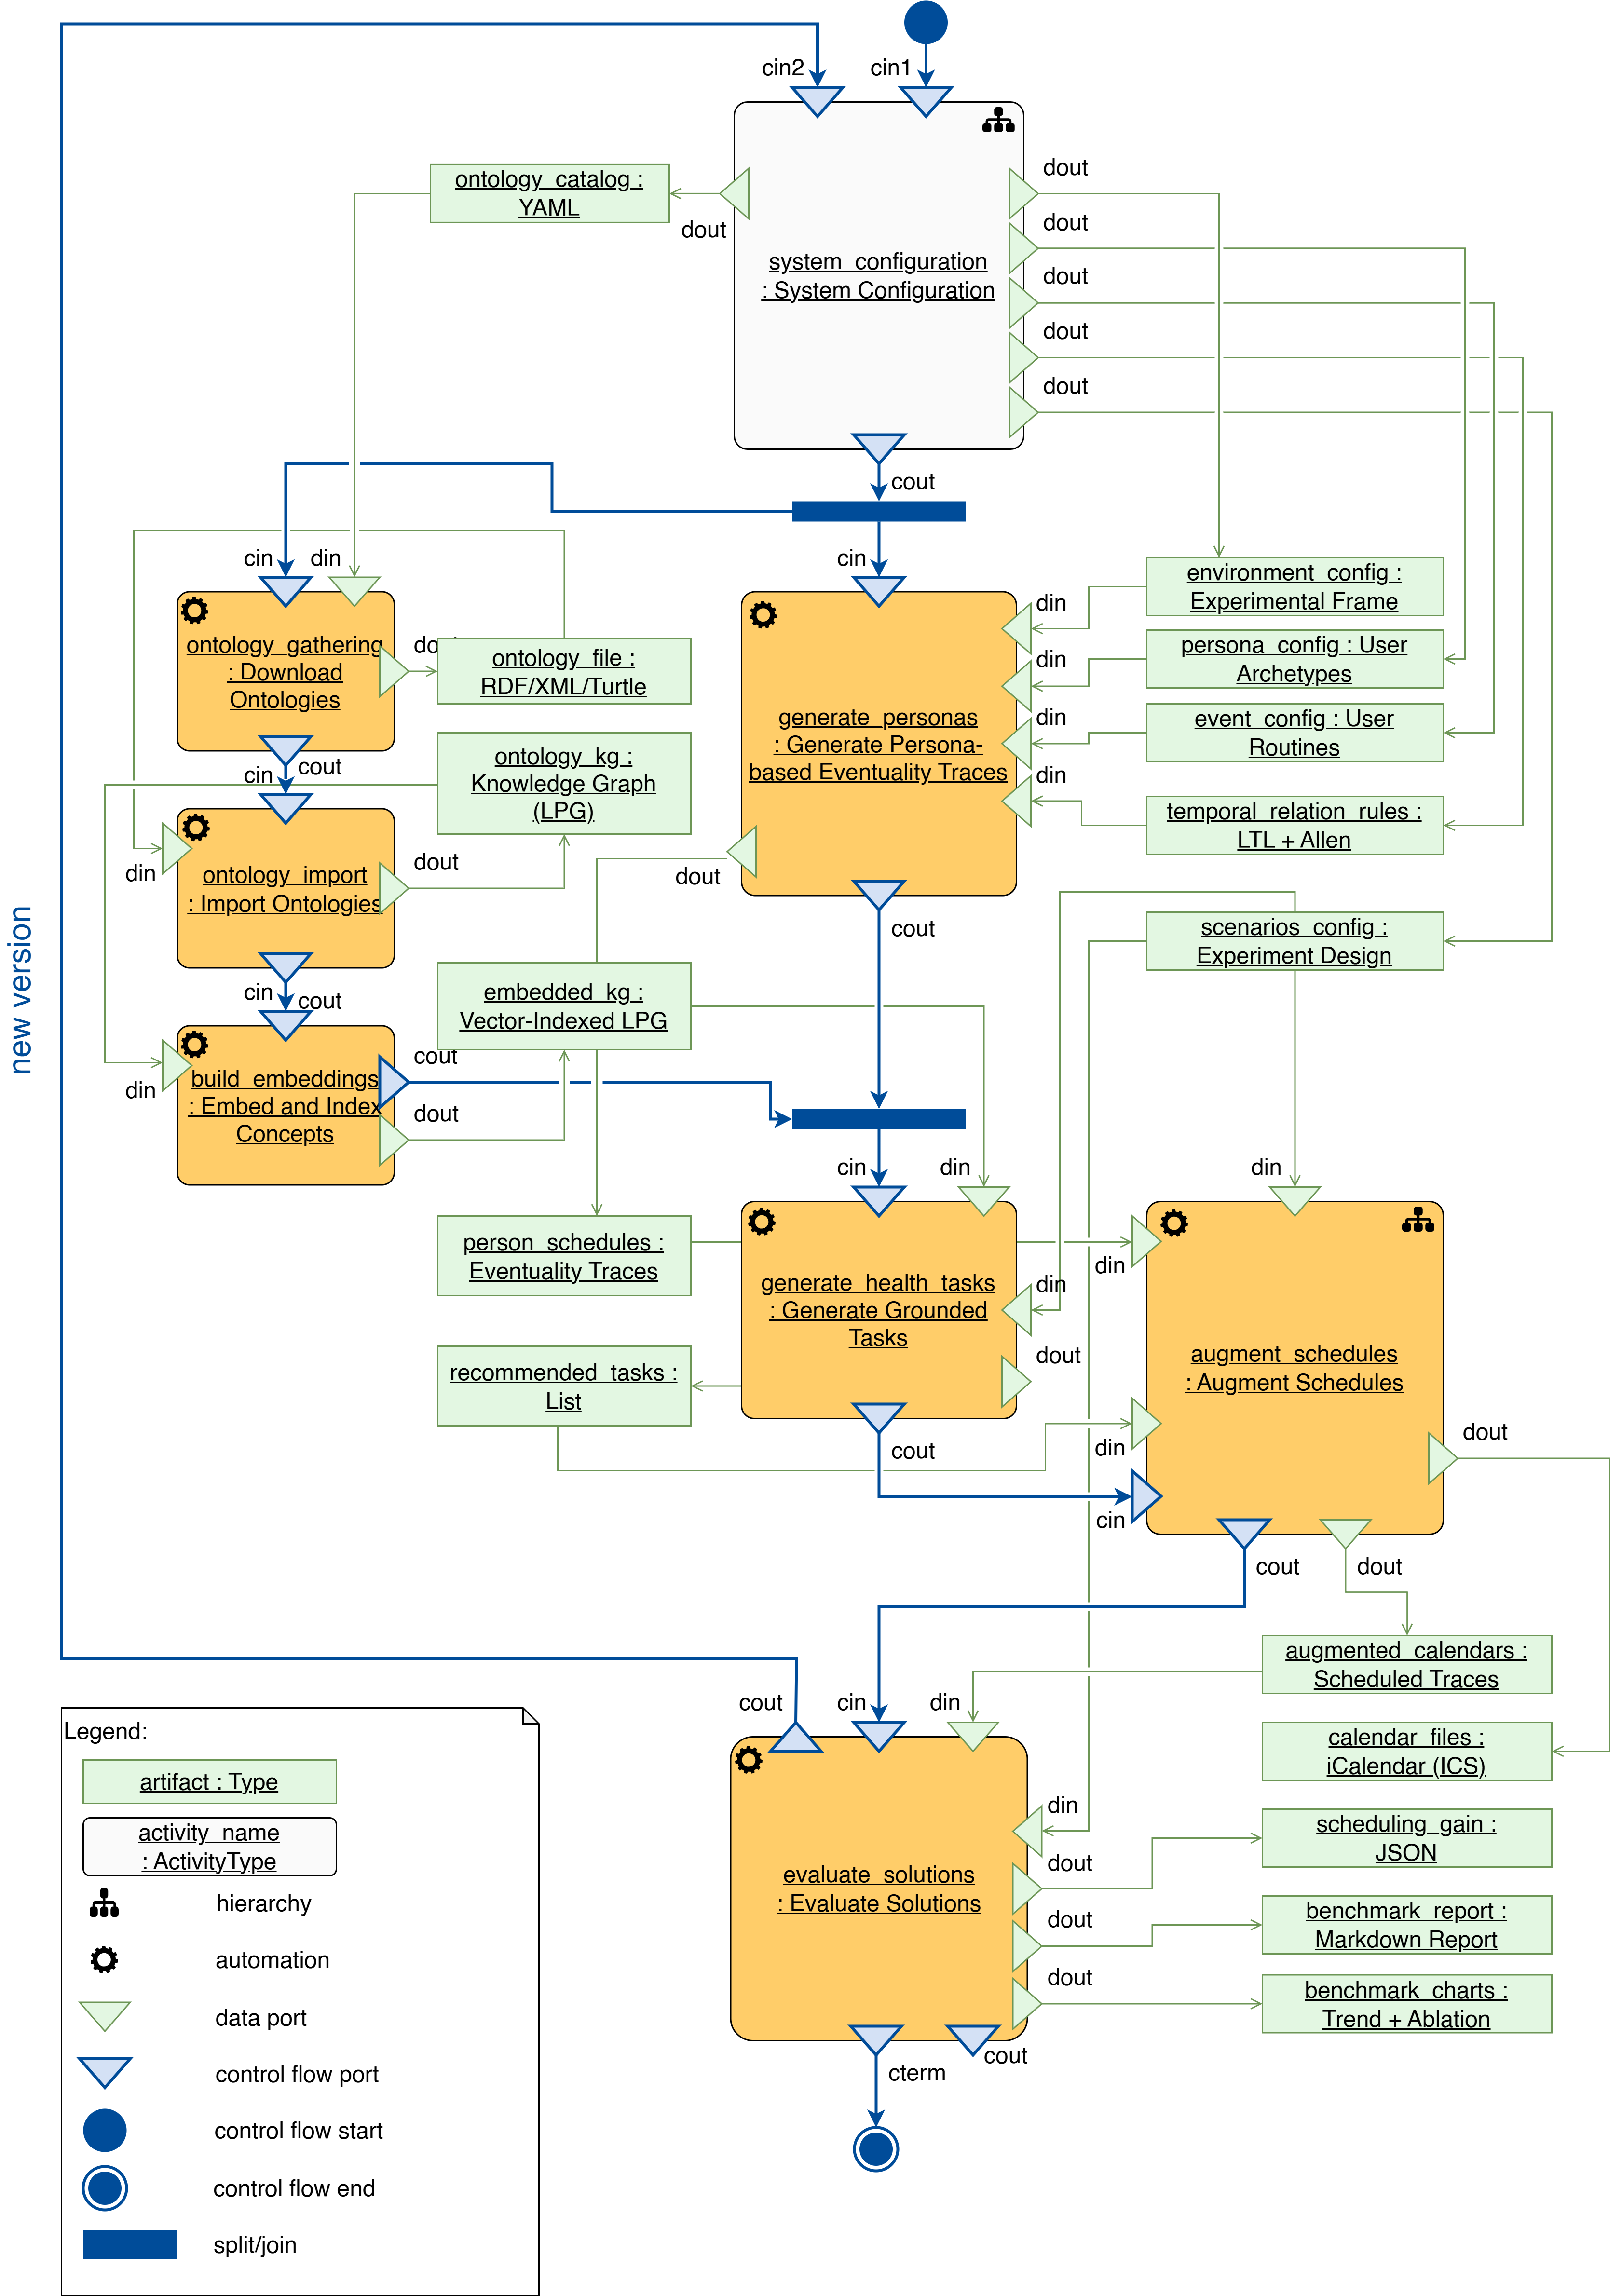
\includegraphics[width=\textwidth]{calendar-bench-ftgpm.png}
    \caption{
         Process model (PM) of \textsc{CalendarBench}.
    }
    \label{fig:workflow}
\end{figure*}
The workflow starts with the composite \textit{System Configuration} activity, where a researcher writes a set of declarative YAML artifacts. The environment file specifies the horizon (e.g. eight weeks) and the time grid (e.g. 10-minute). A persona archetype defines characteristic with sampling distributions. For instance, a person drawn from a full-time employee persona configured for an age from \Colorbox{gray!20}{\lstinline|norm(40, 9)|} clipped to \Colorbox{gray!20}{\lstinline|[22, 65]|} and a weekly workout count from \Colorbox{gray!20}{\lstinline|poisson(3)|}, with a per-episode \Colorbox{gray!20}{\lstinline|default_jitter|} of \Colorbox{gray!20}{\lstinline|time_minutes: 15|} for start times and \Colorbox{gray!20}{\lstinline|duration_minutes: 5|} as random variations. The researchers can specify  eventualities and bound the duration and episode count per timescale and attach a non-stationary pattern of mode \Colorbox{gray!20}{\lstinline|fix|}, \Colorbox{gray!20}{\lstinline|seasonality|}, or \Colorbox{gray!20}{\lstinline|trend|}, such as a gym session with increasing upward trend by 30 minutes per week. The temporal-relation rules employ linear temporal logic (LTL), such as the exclusion \Colorbox{gray!20}{\small$\mathbf{G}\,\lnot(\texttt{sleep}\wedge\texttt{office\_work})$}, for SMT solver based simulations \citep{maas_generating_2026}, and Allen's interval algebra \citep{Allen} for scheduling and evaluation steps.
% , such as the Allen pair rule that specifies a high-intensity activity should be apart from lunch (\Colorbox{gray!20}{\lstinline|event_a: {name: lunch}, event_b: {intensity: [2, 3, 4]}|}, and \Colorbox{gray!20}{\lstinline|admissible relations: {p,P}, buffer: 60|} minutes).
% In the scenario file, the LLM model can be specified for each step (e.g. task-generation, evaluation), the scheduling loss component weights, and source ontologies. 
% Keeping these choices in configuration makes a study reproducible under a fixed seed and versatile without code changes. 
Example configurations are available in \href{https://github.com/MaaniBeigy/calendar-bench}{Github repository}.

The \textit{Download Ontologies} activity reads the catalog and retrieves the source ontologies as TTL/OWL files, including external references for behavior change, food and nutrition, environment, and emotion. We also provide local curated ontologies for human activities \citep{compendium}, our own defined health tasks, and a curated context ontology, based on the imported ontologies from \href{https://bioportal.bioontology.org/ontologies}{bioontology} and \href{https://obofoundry.org/}{obolibrary} databases. The \textit{Import Ontologies} activity loads each file into a Neo4j graph database through the neosemantics extension, which maps vocabulary URIs to graph nodes under a uniqueness constraint on resource identifiers. The \textit{Embed and Index Concepts} activity concatenates the label, synonyms, and definition of each concept, embeds the text with a configurable model (e.g. Qwen3-Embedding-0.6B), and builds a vector index beside the graph, so that the same node is reachable both by typed graph traversal and by approximate nearest-neighbor similarity. The output is a vector-indexed knowledge graph that supports the ontology lookup $\mathcal{O}(\eta,a)$ defined in Section~\ref{sec:math}, so that calendar events, recommended tasks, and context episodes all come from one shared knowledge base.
The \textit{Generate Persona-based Eventuality Traces} step simulates eventualities for each person from the persona archetypes and solves a feasible base weekly calendar with the Z3 SMT solver \citep{deMoura2008Z3:Systems} constrained by the temporal-logic rules compiled into hard constraints, extending the SMT-based behavioral synthesis of Maas et al. \citep{maas_generating_2026}. Non-stationary patterns such as seasonality and trend modify these constraints over the horizon to reflect the evolving nature of human behavior \citep{Barabasi2005}, together with context states. These satisfy the requirements R1 and R2 (table  \ref{tab:req}). The next step is \textit{Generate Grounded Tasks}, which instantiates the $\Gamma$ of Section~\ref{sec:math} by providing a set of self-improvement activities of interest for the simulated persona (e.g. to become more active, or to improve their mental well-being). To satisfy requirement R3 (table  \ref{tab:req}), a vectorCypher retriever seeds candidate concepts by nearest-neighbor search and expands each one along subclass and broader relations and typed neighbors, filtered to the configured domains and levels. Listing~\ref{lst:healthtask-ttl} shows an example task with its grounded context. A configurable LLM model (compatible with OpenAI, Anthropic, or OpenRouter) then proposes the tasks that each cite retrieved URIs, and the activity re-validates to ensure the attributable generation  \citep{zhang_survey_2025}. Surviving labels are paraphrased by a batched LLM call and pass three quality controls on length, emoji use, and a cosine similarity threshold.

The composite \textit{Augment Schedules} activity reads the base calendar, recommended tasks, and scenario design, and runs the augmentations specified in the scenario configuration. The current version of benchmark includes four families: (i) a first-come-first-served greedy gap-filler; (ii) a one-shot LLM planner that plans a full-week schedule; (iii) a PTIME augmenter \citep{Berry2011PTIME:Calendaring}; and (iv) a per-person online deep Q-network trained week by week with a weighted scheduling-gain reward \citep{Mnih2015,Yuan2022}. To meet  requirements R5 and R6 (table  \ref{tab:req}), \textsc{CalendarBench} enables researchers to develop their scheduler methods and add them to the \textit{experiment design} (Figure \ref{fig:workflow}) with the instructions available in \href{https://github.com/MaaniBeigy/calendar-bench}{Github repository}. The \textit{Evaluate Solutions} step scores each augmented calendar with the scheduling loss (Eq.~\ref{eq:loss}), based on scenario configurations, such as \Colorbox{gray!20}{\lstinline|merge_threshold: 0.70|}, \Colorbox{gray!20}{\lstinline|disp_half_life_days: 2|}, and \Colorbox{gray!20}{\lstinline|divide_duration_tolerance_pct: 0.15|}. The results are written as separate artifacts, such as per-run scheduling scores, charts, a benchmark report, and A/B comparison of methods.
 
% A feedback edge runs from \textit{Evaluate Solutions} back to this activity, so that after reading the report and the charts the researcher might revise the script and runs the benchmark again. This loop lets a new method enter the study without changing the rest of the workflow.
% Allen interval-algebra pair rules reserved for evaluation phase (Algorithm~\ref{alg:tempcheck}).

% The intensity component takes the maximum of task difficulty and a MET quartile, whose values derive from the Compendium of Physical Activities \citep{compendium}, and the preference and context-fit components draw on behavior change and self-determination constructs as instances \citep{Prochaska1997TheChange,Ryan2022STheory}. The merging component is scored only at evaluation time by an LLM-as-judge oracle \citep{Zheng2023} that is never exposed to the augmenter, and a benchmark aggregator reports scheduling-gain tables, per-component breakdowns, pairwise deltas, and per-stage cost and latency.

\begin{lstlisting}[caption={An example task with its grounded context.},label={lst:healthtask-ttl}]
hb-tk:write-tomorrow-s-list a hb:MentalWellbeingLevel3 ;
    dcterms:title       "Write Tomorrow's ToDo List" ;
    dcterms:description "Before bed, write down tomorrow's tasks or worries for a few minutes. Close the notebook when you finish." ;
    hb:isConcurrent     true ;
    hb:isDividable      false ;
    hb:matchedActivity  ha-act:sitting-writing-desk-work-typing ;
    hb:contextLink </BCIO_007010> ;  # action planning BCT
    hb:contextLink </MFOEM_000028> ;  # mood_emotion: anxiety
    hb:contextLink </COPPER_2014> ;  # location: home
    ...
\end{lstlisting}

\section{Evaluation}
\label{sec:evaluation}

To demonstrate the capabilities of \textsc{CalendarBench}, we designed an example benchmark experiment, considering previous studies in the literature \citep{jorke_gptcoach_2025,shin_planfitting_2025}. We configured a single full-time employee persona, sampled into eight persons. We crafted a behavior change intervention scenario, where participants are assumed to adopt recommended tasks to improve their physical activity and mental wellbeing. We benchmarked methods over an eight-week horizon on these eight persons, with a fixed seed and a 10-minute time grid. Each person has 10 characteristics (e.g. age, gender, personality traits, and workout frequency) and follows 11 routine activities (e.g. sleep, meals, office work, and exercise) from a catalog of 18 activity types in nine categories (e.g. work, sports, leisure, chores), along with 30 contextual states in eleven categories such as mood, energy, location, and behavior-change state. We defined 57 temporal rules, 38 in LTL and 19 Allen pair rules. We configured the task recommender to provide 20 tasks per person each week, from the physical activity and mental wellbeing domains at difficulty levels two and three. We configured weights for the scheduling loss metric to coverage 0.16, temporal correctness 0.16, dispersion 0.16, preference 0.12, merging 0.12, context fit 0.10, spread 0.10, and division 0.08.


We conducted the experiment with the four augmentation methods of Section~\ref{sec:architecture} with variations of the one-shot LLM planner (single-agent prompt, SAP): a context-blind SAP planner with \texttt{gpt-4o-mini} augmenter; informed SAP planners with  \texttt{gpt-4o-mini} , \texttt{gpt-4.1-mini}, \texttt{gpt-5-mini}, \texttt{gpt-5.4-mini}, and \texttt{claude-opus-4.8}; the task generator and the evaluator replaced with \texttt{gpt-4.1-mini} to be compared with the context-aware \texttt{gpt-4o-mini} SAP planner. The context-aware methods (i.e, informed) read the same five context categories (weather and environment, behavior state, capability and opportunity, goal and intention, and self-determination regulation). The context-blind SAP planner and the PTIME baseline read no context by design. 

Table~\ref{tab:gain} summarizes the average total scheduling gain and its eight components. The informed SAP planner with \texttt{gpt-5-mini} reached the highest total gain (0.853), ahead of \texttt{claude-opus-4.8} (0.802) and the smaller model variants, while the blind and the \texttt{gpt-4o-mini} informed planners underperformed (0.671 and 0.684). Greedy and PTIME covered all tasks ($G_{\text{cov}}=1.000$) because they placed every recommended task, but spread the burden poorly ($G_{\text{spr}}$ of 0.402 and 0.366) and predictably never merged or divided any task ($G_{\text{mrg}}=G_{\text{div}}=0$), which led to their total gain below the SAP models. The SAP methods showed a lower coverage (0.79 to 0.97) but a higher spread (up to 0.97) and non-zero merging and division scores. Temporal consistency ($G_{\text{cal}}\approx0.96$) and intensity dispersion ($G_{\text{disp}}\approx0.999$) were high for all methods, so the methods performed differently mainly in coverage, spread, merging, division, and context fit. Merging was hard for the smaller models but increased with SOTA LLM capabilities, reaching 0.769 for \texttt{gpt-5-mini}, which indicates that semantically correct co-scheduling is one of the hardest and most expensive dimensions of the personal scheduling benchmark.

As expected, context awareness had a large impact on SAP model performance, so compared to the blind planner, the informed planner could double the context fit (0.187 to 0.411) at a negligible cost increase (\$0.14 to \$0.18 per scenario). Along the model axis, a stronger augmenter improved the total gain (Table~\ref{tab:gain}) but its cost increased dramatically, from \$0.18 for \texttt{gpt-4o-mini} to \$0.36 for \texttt{gpt-5-mini} and \$5.49 for \texttt{claude-opus-4.8}. Swapping only the evaluator or the task generator to \texttt{gpt-4.1-mini} barely changed the total gain, confirming that these steps are less dependent on the LLM model capabilities in the overall benchmarking. 

Figure~\ref{fig:weekly} compares the average weighted scheduling gain of different methods per week. The non-learning methods stay flat throughout the horizon (slope magnitudes at most 0.004), while the online DQN (context-awareness identical to informed SAP models) started low (0.135 in week one), showed improvement to the range of the heuristic baselines by week three (0.585), and was the only run with a clearly positive slope ($\Delta$ of 0.447 from the first to the last week). All eight persons converged. The RL agent therefore learns a usable policy within the horizon from its scheduling-gain reward, but its average total gain (0.625) stays below the informed LLM planners over eight weeks.
\begin{table}[t]
\centering
\caption{Average total scheduling gain ($G$) and its eight components on the example experiment. SAP stands for single-agent prompt one-shot LLM planner, \emph{blind} planner reads no context, and a row marked with a model (e.g. \texttt{aug 5-mini}, \texttt{gen 4.1-mini}) used that model at that stage instead of baseline \texttt{gpt-4o-mini}. The legs are coverage, calendar consistency, preference, intensity dispersion, merging, spread, splitting, and context fit.}
\label{tab:gain}
\setlength{\tabcolsep}{3pt}
\footnotesize
\begin{tabular}{lrrrrrrrrr}
\toprule
Method & $G$ & $G_{\text{cov}}$ & $G_{\text{cal}}$ & $G_{\text{pref}}$ & $G_{\text{disp}}$ & $G_{\text{mrg}}$ & $G_{\text{spr}}$ & $G_{\text{div}}$ & $G_{\text{ctx}}$ \\
\midrule
SAP, blind          & 0.671 & 0.824 & 0.964 & 0.809 & 0.999 & 0.118 & 0.817 & 0.164 & 0.187 \\
SAP, informed       & 0.684 & 0.837 & 0.965 & 0.782 & 0.999 & 0.016 & 0.853 & 0.175 & 0.411 \\
SAP, aug 4.1-mini   & 0.743 & 0.789 & 0.959 & \textbf{0.843} & 0.999 & 0.440 & 0.902 & 0.202 & 0.436 \\
SAP, aug 5-mini     & \textbf{0.853} & 0.969 & 0.954 & 0.792 & 0.999 & \textbf{0.769} & 0.913 & 0.608 & \textbf{0.579} \\
SAP, aug 5.4-mini   & 0.753 & 0.872 & 0.964 & 0.783 & 0.999 & 0.319 & \textbf{0.971} & 0.324 & 0.445 \\
SAP, aug opus-4.8   & 0.802 & 0.915 & 0.963 & 0.827 & 0.999 & 0.559 & 0.795 & \textbf{0.635} & 0.451 \\
SAP, eval 4.1-mini  & 0.696 & 0.827 & 0.963 & 0.795 & 0.999 & 0.066 & 0.839 & 0.251 & 0.425 \\
SAP, gen 4.1-mini   & 0.666 & 0.832 & \textbf{0.971} & 0.747 & 0.999 & 0.025 & 0.844 & 0.018 & 0.396 \\
Greedy              & 0.651 & \textbf{1.000} & 0.968 & 0.831 & 0.999 & 0.000 & 0.402 & 0.000 & 0.367 \\
PTIME               & 0.627 & \textbf{1.000} & 0.963 & 0.805 & 0.999 & 0.000 & 0.366 & 0.000 & 0.200 \\
RL (online DQN)     & 0.625 & 0.819 & 0.966 & 0.729 & 0.998 & 0.000 & 0.584 & 0.000 & 0.339 \\
\bottomrule
\end{tabular}
\end{table}

\begin{figure*}[!h]
\centering

\includegraphics[width=0.95\textwidth]{cross_augmenter_weekly.png}
\caption{Average weighted scheduling gain per week for the example benchmark experiment.}
\label{fig:weekly}
\end{figure*}


\section{Conclusion}
\label{sec:conclusion}
In this paper, we introduce a benchmark framework with a repository of available methods as an ongoing effort to address personal scheduling problems. \textsc{CalendarBench} addresses an important requirement for designers, developers, and researchers in the extensive domains of productivity and time management, lifestyle promotion, and health behavior change. Based on the advantages and shortcomings of related work on personal scheduling (e.g. PTIME \citep{Berry2011PTIME:Calendaring}, CMRadar \citep{Modi2005CMRadar:Management}, CP-SAT \citep{cpsat}) and earlier calendaring and planning benchmarks \citep{zheng_natural_2024,xie_travelplanner_2024,valmeekam_planbench_2023}, we developed a versatile benchmarking framework for experimenting with a variety of scheduling techniques on evolving user calendars with several human-centric contexts and objectives at once. We demonstrated such capabilities with an example benchmark experiment that compares a greedy heuristic, PTIME, one-shot singe-agent planner with SOTA LLMs, and online DQN RL schedulers. 

Our work also has some limitations. By design, we covered only the single-user setting, so multi-user negotiation, shared-resource planning, and competitive scheduling are outside our scope. Curating ontologies and manually writing the configuration files for simulation scenarios and personas can be time-consuming, which motivates coupling this benchmark with collaborative approaches \citep{maas_generating_2026}. The present example experiment used a single persona with few instances, and provisional LLM prompts for scheduling. Therefore, even though our findings are illustrative, they remain limited to the models used and the simulation configuration. Validation with domain experts, testing on more diverse personas and models, and the hybrid multi-agent schedulers are the natural next steps.

\begin{credits}
\subsubsection{\ackname}
The authors used an AI coding assistant (Claude Code, Anthropic) to help develop and document parts of the source code; it was not used to generate the text of this paper. Writefull plugin of overleaf was used for grammar and spell checking.

\subsubsection{\discintname}
The authors have no competing interests to declare that are relevant to the content of this article.
\end{credits}


\bibliographystyle{splncs04}  % abbrvnat plainnat
\bibliography{references}
\end{document}
